%------------------
% Pygame Presentation
% for Python User Group Freiburg
% December 11th, 2013
%
% Felix Hoffmann
% about.me/felixhoffmann
%------------------



%\documentclass{beamer}
\documentclass[handout]{beamer}   %uncomment for handout
\usetheme{default}

\usepackage{comment}
\usepackage{color}
\usepackage{underscore}
\usepackage{hyperref}

\usepackage{minted}


\newminted{python}{fontsize=\scriptsize, linenos,
               		numbersep=8pt,
               		gobble=4,
               		frame=lines,
					bgcolor=bg,
               		framesep=3mm}         		
               		
\newenvironment{gcode}{\textcolor{tg}{\texttt{}{}}}   

%suggested by ilpssun, %http://tex.stackexchange.com/questions/48473/best-way-to-give-sources-of-images-used-in-a-beamer-presentation 
\usepackage[absolute,overlay]{textpos}

\setbeamercolor{framesource}{fg=gray}
\setbeamerfont{framesource}{size=\tiny}

\newcommand{\source}[1]{\begin{textblock*}{4cm}(8.7cm,8.6cm)
    \begin{beamercolorbox}[ht=0.5cm,right]{framesource}
        \usebeamerfont{framesource}\usebeamercolor[fg]{framesource} Source: {#1}
    \end{beamercolorbox}
\end{textblock*}}




            		
               		               		
\title{Pygame!}
\subtitle{Python User Group Freiburg}
\author[Felix Hoffmann]{Felix Hoffmann}
\institute{\url{http://about.me/felixhoffmann}}
\date{\today}        		


\begin{document}

\definecolor{bg}{rgb}{0.95,0.95,0.95}
\definecolor{tg}{rgb}{0.35,0.35,0.35}


%----------- titlepage ----------------------------------------------%



%----------- titlepage ----------------------------------------------%

\begin{frame}[plain]
  \titlepage
\end{frame}


%----------- slide --------------------------------------------------%


\begin{frame}[plain]
\begin{center}

\includegraphics[width=0.6\textwidth]{img/pygame.png}
\vspace{1cm}
\url{http://www.pygame.org}\\
\vspace{1.4cm}
Pygame is a Python wrapper around the SDL library (Simple DirectMedia Layer) with a few unique libraries with an emphasis on game programming, written by Pete Shinners.
\end{center}
\end{frame}


\begin{frame}

\frametitle{From the FAQ}

\begin{itemize}

\item[] \textbf{Does not require OpenGL} 
\item[] Uses either opengl, directx, windib, X11, linux frame buffer, and many other different backends... including an ASCII art backend!
\item[]
\item[] \textbf{Truly portable}
\item[] Supports Linux, Windows, Windows CE, BeOS, MacOS, Mac OS X, FreeBSD, NetBSD, OpenBSD, BSD/OS, Solaris, IRIX, and QNX \dots
\item[]
\item[] \textbf{Silliness built in!}
\end{itemize}
\end{frame}





\defverbatim[colored]\simplePygame{
\begin{pythoncode}
               	
    import pygame

    pygame.init()
    screen = pygame.display.set_mode((640, 480))

    color = [(0,0,0),(255,255,255)]
    running = True

    while running:
        for event in pygame.event.get():
            if event.type == pygame.QUIT:
                running = False
            if event.type == pygame.KEYDOWN:
                color[0], color[1] = color[1],color[0]
            
        screen.fill(color[0])
        pygame.display.flip()
        
\end{pythoncode}   
}
\begin{frame}
\frametitle{A simple Pygame example}
\simplePygame  

\pause
\medskip

\textcolor{tg}{\texttt{01-simple_pygame.py}}  
\end{frame}


\defverbatim[colored]\importPygame{
\begin{minted}[xleftmargin = 10mm]{python}
import pygame 
\end{minted}
}
\defverbatim[colored]\importLocals{
\begin{minted}[xleftmargin = 10mm]{python}
from pygame.locals import *
\end{minted}
}
\defverbatim[colored]\initPygame{
\begin{minted}[xleftmargin = 10mm]{python}
pygame.init()
\end{minted}
}
\begin{frame}
\frametitle{What each element does: Importing \& Initializing}

\importPygame
to import the Pygame module.
\pause
\medskip
\importLocals
Optional. Puts limited set of constant and function in the \textbf{global namespace}.  
\medskip
\pause
\initPygame
to initialize Pygame's modules (e.g. \texttt{pygame.font}). Not always needed, but recommended in \textit{any} case.

\end{frame}


%---------------------------------------------------------------------

\defverbatim[colored]\setScreen{
\begin{minted}[xleftmargin = 10mm]{python}
screen = pygame.display.set_mode((640, 480))
\end{minted}
}
\begin{frame}[fragile]
\frametitle{What each element does: Setting Window \& Screen}
\setScreen

initializes a \textbf{window} with dimensions $640 \times 480$ and returns the \textbf{screen object}.
\pause
\bigskip

Everything to be displayed needs to be drawn on the \textcolor{tg}{\texttt{screen}}.
\end{frame}


%---------------------------------------------------------------------


\defverbatim[colored]\initWindow{
\begin{pythoncode}
               	
    import pygame

    pygame.init()
    screen = pygame.display.set_mode((640, 480))
        
\end{pythoncode}  
}
\begin{frame}
\frametitle{Initializing a Pygame window}
Together:
\medskip
\initWindow
\pause
\bigskip

\textcolor{tg}{\texttt{02-window.py}}

\end{frame}


%---------------------------------------------------------------------


\begin{frame}[fragile]
\frametitle{Initializing a Pygame window - Extended}
\begin{pythoncode}
               	
    import pygame

    pygame.init()
    screen = pygame.display.set_mode((640, 480))

    running = True
    while running:
        for event in pygame.event.get():
            if event.type == pygame.QUIT:
                running = False
        
\end{pythoncode}        
\end{frame}
%--------------------------------------------------------------------

\defverbatim[colored]\mainLoop{
\begin{pythoncode}

    running = True
    while running:
        for event in pygame.event.get():
            if event.type == pygame.QUIT:
                running = False
            if event.type == pygame.KEYDOWN:
                color[0], color[1] = color[1],color[0]
            
        screen.fill(color[0])
        pygame.display.flip()
        
\end{pythoncode}  
}
\begin{frame}
\frametitle{What each element does: The Main Loop}

\mainLoop
  
\medskip

is the \textbf{main loop} of the game.
\pause
\begin{itemize}
\item listen to events $\rightarrow$ respond
\pause
\item proceed the game
\pause
\item draw on the screen
\pause
\item stop when done
\end{itemize}
\end{frame}




%---------------------------------------------------------------------
\begin{comment}
\begin{frame}[plain]
\begin{center}
\Huge
How do I do this all myself?
\end{center}
\end{frame}
\end{comment}
%---------------------------------------------------------------------

\defverbatim[colored]\mainFrame{
\begin{pythoncode}
               	
    import pygame

    pygame.init()
    screen = pygame.display.set_mode((640, 480))

    running = True
    while running:
        for event in pygame.event.get():
            if event.type == pygame.QUIT:
                running = False
            if event.type == pygame.KEYDOWN:
                react_to_user_input()
            
        do_things_the_game_does()
        draw_everything_on_the_screen()
        
\end{pythoncode} 
}

\begin{frame}
\frametitle{A framework for your Pygames}

\mainFrame
 
\pause
\textbf{Next}:
\begin{itemize}
\item Drawing
\pause
\item User Input
\pause
\item Game Events
\end{itemize}      
\end{frame}

%---------------------------------------------------------------------

\begin{frame}[plain]
\begin{center}
\Huge
Drawing
\end{center}
\end{frame}

%---------------------------------------------------------------------

\defverbatim[colored]\screenFill{
\begin{pythoncode}
    blue = (0,0,255)
    screen.fill(blue)
    pygame.display.flip()
\end{pythoncode}
}

\defverbatim[colored]\drawCircle{
\begin{pythoncode}
    red = (255,0,0)
    # position (320,240), radius = 50
    pygame.draw.circle(screen, red, (320,240), 50)
\end{pythoncode}
}

\begin{frame}
\frametitle{Drawing on the screen I}
Filling the screen with a color:

\screenFill
\pause
After all drawing is done, call \textcolor{tg}{\texttt{display.flip()}} to \textbf{update} the display.\\
\bigskip
\medskip
\pause
Use pygame.draw to draw geometric shapes. A circle:
\drawCircle

\end{frame}

%---------------------------------------------------------------------

\defverbatim[colored]\redLine{
\begin{pythoncode}
    red = (255,0,0)
    pygame.draw.line(screen, red, (10,50),(30,50),10)
\end{pythoncode}
}


\begin{frame}
\frametitle{Drawing on the screen II}

Geometric shapes available for \textcolor{tg}{\texttt{pygame.draw}}:
\medskip
\begin{itemize}
\pause
\item[] \textcolor{tg}{\texttt{circle(Surface, color, pos, radius, width$=$0)}}
\pause
\item[] \textcolor{tg}{\texttt{\mbox{polygon(Surface, color, pointlist, width$=$0)}}}
\pause
\item[] \textcolor{tg}{\texttt{line(Surface, color, start, end, width$=1$)}}
\pause
\item[] \textcolor{tg}{\texttt{rect(Surface, color, Rect, width$=$0)}}
\pause
\item[] \textcolor{tg}{\texttt{ellipse(Surface, color, Rect, width$=$0)}}
\end{itemize}
\bigskip
\medskip
\pause
Example:
\redLine

\end{frame}

%---------------------------------------------------------------------

\defverbatim[colored]\defColor{
\begin{minted}[xleftmargin = 10mm]{python}
    gray = (200,200,200)
    #(red, green, blue)
\end{minted}
}

\begin{frame}
\frametitle{Drawing on the screen - Colors}

Defining a color
\defColor
\bigskip
\pause
Use for example \textcolor{tg}{\texttt{colorpicker.com}}:
\begin{center}
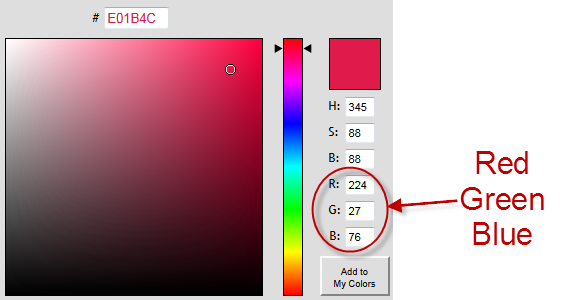
\includegraphics[width=0.8\textwidth]{img/colorpicker.png}
\source{Paul Craven, \href{http://programarcadegames.com/}{programarcadegames.com/}}
\end{center}
\end{frame}

%---------------------------------------------------------------------

\defverbatim[colored]\defPos{
\begin{minted}[xleftmargin = 10mm]{python}
    P = (11,9)
    #(x-axis, y-axis)
\end{minted}
}
\begin{frame}
\frametitle{Drawing on the screen - Positions}

Defining a position:
\defPos
\bigskip
\pause
To the reference coordinate system
\begin{center}
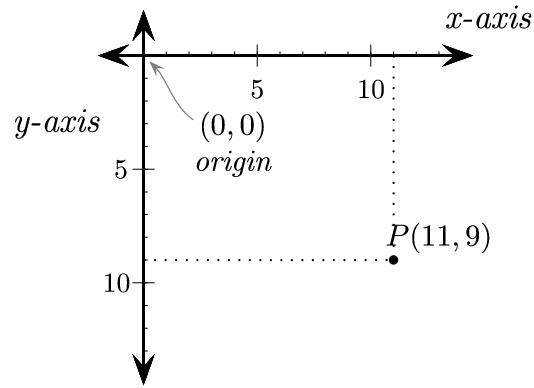
\includegraphics[width=0.6\textwidth]{img/coordinates.png}
\source{Paul Craven, \href{http://programarcadegames.com/}{programarcadegames.com/}}
\end{center}
\end{frame}

%---------------------------------------------------------------------

\defverbatim[colored]\rectCode{
\begin{minted}[xleftmargin = 10mm]{python}
pygame.Rect(left, top, width, height)
\end{minted}
}
\defverbatim[colored]\drawRect{
\begin{pythoncode}
    box = pygame.Rect(10, 10, 100, 40)
    pygame.draw.rect(screen, blue, box)
    #draws at (10,10) rectangle of width 100, height 40
\end{pythoncode}
}
\begin{frame}
\frametitle{Drawing on the screen - Rects}
\rectCode
to create a Rect. 
\pause
\vspace{0.4cm}

\drawRect
\pause 
Rect anchors:
\begin{itemize}
\item[]    \textcolor{tg}{\texttt{top, left, bottom, right}}
\item[]    \textcolor{tg}{\texttt{topleft, bottomleft, topright, bottomright}}
\item[]    \textcolor{tg}{\texttt{midtop, midleft, midbottom, midright}}
\item[]    \textcolor{tg}{\texttt{center, centerx, centery}}
\item[]    \textcolor{tg}{\texttt{size, width, height}}
\item[]    \textcolor{tg}{\texttt{w,h}}
\end{itemize}

\end{frame}



%---------------------------------------------------------------------

\defverbatim[colored]\drawEx{
\begin{pythoncode}
               	
    import pygame

    pygame.init()
    screen = pygame.display.set_mode((640, 480))

    white = (255,255,255)
    blue = (0,0,255)

    running = True
    while running:
        for event in pygame.event.get():
            if event.type == pygame.QUIT:
                running = False

        screen.fill(white)
        pygame.draw.circle(screen, blue, (320,240), 100)    
        # position (320,240), radius = 100

        pygame.display.flip()
        
\end{pythoncode}
}

\begin{frame}
\frametitle{A full drawing example}

\drawEx
\pause
\textcolor{tg}{\texttt{04-drawing.py}}.       
\end{frame}


%---------------------------------------------------------------------

\begin{frame}[plain]
\begin{center}
\Huge
User Input
\end{center}
\end{frame}

%---------------------------------------------------------------------

\defverbatim[colored]\pyEvent{
\begin{minted}[xleftmargin = 10mm]{python}
pygame.event.get()
\end{minted}
}
\defverbatim[colored]\forEvent{
\begin{pythoncode*}{fontsize=\small}
    for event in pygame.event.get():
        if event.type == YourEvent:
            react_to_your_event()
\end{pythoncode*}
}
\defverbatim[colored]\pygameQuit{
\begin{minted}[xleftmargin = 10mm]{python}
pygame.Rect(left, top, width, height)
\end{minted}
}
\begin{frame}
\frametitle{Events}
get all events in Pygame's event queue
\pyEvent
\pause
\bigskip
\medskip

usually used as

\bigskip
 
\forEvent

\end{frame}



\begin{frame}
\frametitle{Event types}

Some of the most important event types are:
\medskip
\begin{itemize}
\pause
\item[] \textcolor{tg}{\texttt{pygame.QUIT}} 
\pause
\item[] \textcolor{tg}{\texttt{pygame.KEYDOWN}}
\pause
\item[] \textcolor{tg}{\texttt{pygame.KEYUP}}
\pause
\item[] \textcolor{tg}{\texttt{pygame.USEREVENT}}
\pause
\end{itemize}
\bigskip
\medskip
\pause

With 
\importLocals
from earlier, prefix \textcolor{tg}{\texttt{pygame}} isn't needed.
\end{frame}


\defverbatim[colored]\keydown{
\begin{pythoncode*}{fontsize=\small}
    while running:
        for event in pygame.event.get():
            if event.type == KEYDOWN:
                react_to_key()
\end{pythoncode*}
}
\defverbatim[colored]\escapeDown{
\begin{pythoncode*}{fontsize=\small}
    for event in pygame.event.get():
        if event.type == KEYDOWN:
            if event.key == K_ESCAPE:
                running = False
\end{pythoncode*}
}
\begin{frame}
\frametitle{Events}
React to \textcolor{tg}{\texttt{KEYDOWN}} event:
\medskip
\keydown
\pause
\bigskip

Which key?  \pause $\rightarrow$ if event type is \textcolor{tg}{\texttt{KEYDOWN}} or \textcolor{tg}{\texttt{KEYUP}} event has attribute \textbf{key}.
\medskip
\escapeDown
\end{frame}

\begin{frame}
\frametitle{Pygame Keys}
Some of the most important keys are:
\medskip
\begin{itemize}
\pause
\item[] \textcolor{tg}{\texttt{K_RETURN}} 
\item[] \textcolor{tg}{\texttt{K_SPACE}}
\item[] \textcolor{tg}{\texttt{K_ESCAPE}}
\item[] \textcolor{tg}{\texttt{K_UP, K_DOWN, K_LEFT, K_RIGHT}}
\item[] \textcolor{tg}{\texttt{K_a, K_b, ...}}
\item[] \textcolor{tg}{\texttt{K_0, K_1, ...}}
\pause
\end{itemize}
\bigskip
\medskip
\pause


Full list of keys: \url{http://www.pygame.org/docs/ref/key.html}
\end{frame}




\defverbatim[colored]\getKeys{
\begin{minted}[xleftmargin = 10mm]{python}
key = pygame.key.get_pressed()
\end{minted}
}
\defverbatim[colored]\moveUP{
\begin{minted}[xleftmargin = 10mm]{python}
if key[pygame.K_UP]:
    move_up()    
\end{minted}
}
\begin{frame}
\frametitle{Getting continuous input}

\textcolor{tg}{\texttt{KEYDOWN}} is a unique event. 
\pause
\bigskip
\getKeys
to get keys currently pressed.
\pause
\bigskip
\moveUP
to check and react on a specific key.
\end{frame}


\defverbatim[colored]\uiExamp{
\begin{pythoncode*}{fontsize=\footnotesize}
    color = [0,0,0]

    while running:
        for event in pygame.event.get():
            if event.type == pygame.QUIT:
                running = False
            if event.type == KEYDOWN and event.key == K_SPACE:
                color = [0,0,0]
        
        keys = pygame.key.get_pressed()
        if keys[K_UP]:
            color = [(rgb+1)%256 for rgb in color]

        screen.fill(color)
        pygame.display.flip()
\end{pythoncode*}
}
\begin{frame}
\frametitle{A user input example}
\uiExamp
\pause
\medskip
\textcolor{tg}{\texttt{05-user_input.py}}

\end{frame}


\begin{frame}[plain]
\begin{center}
\Huge
Pygame's Clock
\end{center}
\end{frame}


\defverbatim[colored]\clock{
\begin{minted}[xleftmargin = 10mm]{python}
clock = pygame.time.Clock()
\end{minted}
}
\defverbatim[colored]\clockTick{
\begin{minted}[xleftmargin = 10mm]{python}
clock.tick(60) #limit to 60 fps
\end{minted}
}
\begin{frame}
\frametitle{Limiting the frames per second}

\pause
\clock
to initialize the clock.
\pause
\bigskip
\vspace{1cm}

In your main loop call
\clockTick

\end{frame}


\defverbatim[colored]\clockExamp{
\begin{pythoncode*}{fontsize=\footnotesize}
    clock = pygame.time.Clock()

    while running:
        for event in pygame.event.get():
            if event.type == pygame.QUIT:
                running = False
            if event.type == KEYDOWN and event.key == K_SPACE:
                color = [0,0,0]
        
        keys = pygame.key.get_pressed()
        if keys[K_UP]:
            color = [(rgb+1)%256 for rgb in color]

        screen.fill(color)
        pygame.display.flip()

        clock.tick(60)
\end{pythoncode*}
}
\begin{frame}
\frametitle{Clock example}
\clockExamp
\pause
\medskip
\textcolor{tg}{\texttt{06-clock.py}}

\end{frame}













\begin{frame}[plain]
\begin{center}
\Huge
Game Events \\
\end{center}
\end{frame}

%---------------------------------------------------------------------

%---------------------------------------------------------------------

\begin{frame}
\frametitle{Sprites}

Pygame's \textbf{sprite class} gives convenient options for handling interactive graphical objects. \\
\medskip
\pause
If you want to draw \textbf{and} move (or manipulate) and object, make it a sprite.
\pause
\bigskip

\textbf{Sprites} 
\begin{itemize}
\item[] can be grouped together 
\item[] are easily drawn to a surface (even as a group!)
\item[] have an update method that can be modified
\item[] have collision detection
\end{itemize}
\end{frame}

%---------------------------------------------------------------------

\defverbatim[colored]\spriteExample{
\begin{pythoncode*}{fontsize=\footnotesize}

    class SpriteExample(pygame.sprite.Sprite):

        def __init__(self):
            pygame.sprite.Sprite.__init__(self)

            self.image = #image
            self.rect = #rect

        def update(self):
            pass

\end{pythoncode*}
}
\begin{frame}
\frametitle{Basic Sprite}

\spriteExample

\end{frame}



\defverbatim[colored]\spriteFromImage{
\begin{pythoncode*}{fontsize=\footnotesize}

    class SpriteExample(pygame.sprite.Sprite):

        def __init__(self):
            pygame.sprite.Sprite.__init__(self)

            self.image = pygame.image.load('local_img.png')
            self.rect = self.image.get_rect()
            self.rect.topleft = (80,120)

        def update(self):
            pass

\end{pythoncode*}
}
\begin{frame}
\frametitle{Sprite from a local image}

\spriteFromImage

\end{frame}



\defverbatim[colored]\spriteRectangle{
\begin{pythoncode*}{fontsize=\footnotesize}

    class Rectangle(pygame.sprite.Sprite):

        def __init__(self):
            pygame.sprite.Sprite.__init__(self)
            self.image = pygame.Surface([200, 50])
            self.image.fill(blue)
            self.rect = self.image.get_rect()
            self.rect.top, self.rect.left = 100, 100

        def update(self):
            pass

\end{pythoncode*}
}
\begin{frame}
\frametitle{Self-drawn sprites: Rectangle}

\spriteRectangle

\end{frame}

\begin{comment}
\defverbatim[colored]\spriteTrans{
\begin{pythoncode*}{fontsize=\footnotesize}

    def __init__(self):
        pygame.sprite.Sprite.__init__(self)

        self.image = pygame.Surface([100, 100], pygame.SRCALPHA, 32)
        pygame.draw.circle(self.image, blue, (50, 50), 50)
        self.image = self.image.convert_alpha()

        self.rect = self.image.get_rect()
        self.rect.center = [320,240]

\end{pythoncode*}
}
\begin{frame}
\frametitle{Self-drawn sprites: Transparency}

By default \textcolor{tg}{\texttt{pygame.Surface}} is black. For transparency:
\vspace{0.6cm}

\spriteTrans

\end{frame}
\end{comment}

\defverbatim[colored]\colorRectangle{
\begin{pythoncode*}{fontsize=\footnotesize}

    class Rectangle(pygame.sprite.Sprite):

        def __init__(self, color):
            pygame.sprite.Sprite.__init__(self)
            self.image = pygame.Surface([200, 50])
            self.image.fill(color)
            self.rect = self.image.get_rect()
            self.rect.top, self.rect.left = 100, 100

        def update(self):
            pass

\end{pythoncode*}
}
\defverbatim[colored]\initCR{
\begin{pythoncode*}{fontsize=\footnotesize}

    white, blue = (255,255,255), (0,0,255)
    
    white_rect = Rectangle(white)
    blue_rect = Rectangle(blue)

\end{pythoncode*}
}
\begin{frame}
\frametitle{Sprites: A reminder about classes}

\colorRectangle
\pause
\vspace{0.2cm}
\initCR

\end{frame}


\defverbatim[colored]\spriteGroup{
\begin{minted}[xleftmargin = 10mm]{python}
new_sprite_group = pygame.sprite.Group(sprite1)
\end{minted}
}
\defverbatim[colored]\addingGroup{
\begin{minted}[xleftmargin = 10mm]{python}
new_sprite_group.add(sprite2)
\end{minted}
}
\defverbatim[colored]\groupUD{
\begin{pythoncode*}{fontsize=\footnotesize}
    
    #inside main loop:

    new_sprite_group.update() #game events
    new_sprite_group.draw()   #drawing  

\end{pythoncode*}
}
\begin{frame}
\frametitle{Sprite groups}

\pause
\spriteGroup
to create a new sprite group containing sprite \textcolor{tg}{\texttt{sprite1}}. \\
\pause
\bigskip

\addingGroup
to add another sprite later.
\pause 
\bigskip

Group updating and drawing:
\medskip
\groupUD

\end{frame}




\defverbatim[colored]\frameSpr{
\begin{pythoncode*}{fontsize=\footnotesize}
    
    class NewSprite(pygame.sp...
        #defining a new sprite

    newsprite = NewSprite()
    sprites = pygame.sprite.Group()
    sprites.add(newsprite)   
    
    while running:
        for event in ...

        sprites.update() #game events
        sprites.draw()
        pygame.display.flip()

\end{pythoncode*}
}
\begin{frame}
\frametitle{Framework for working with sprite groups}

\frameSpr

\end{frame}



\defverbatim[colored]\spriteCirc{
\begin{pythoncode*}{}
    
    class Circle(pygame.sprite.Sprite):
        def __init__(self):
            pygame.sprite.Sprite.__init__(self)
            self.image = pygame.Surface([100, 100])
            pygame.draw.circle(self.image, blue, (50, 50), 50)
            self.rect = self.image.get_rect()
            self.rect.center = [320,240]

    def draw(sprites):
        screen.fill(white)
        sprites.draw(screen)
        pygame.display.flip()

    circle = Circle()
    sprites = pygame.sprite.Group(circle)

    while running:
        sprites.update() 
        draw(sprites)

\end{pythoncode*}
}
\begin{frame}
\frametitle{Sprite groups: working example}

\spriteCirc
\pause
\medskip

\textcolor{tg}{\texttt{07-sprite-circle.py}}
\end{frame}


\defverbatim[colored]\transpCirc{
\begin{pythoncode*}{}
    
    class Circle(pygame.sprite.Sprite):
        def __init__(self):
            pygame.sprite.Sprite.__init__(self)
            self.image = pygame.Surface([100, 100], pygame.SRCALPHA, 32)
            pygame.draw.circle(self.image, blue, (50, 50), 50)
            self.image = self.image.convert_alpha()

\end{pythoncode*}
}
\begin{frame}
\frametitle{Working example: Transparency}
By default \textcolor{tg}{\texttt{pygame.Surface}} is black. For transparency:
\vspace{0.4cm}
\transpCirc
\pause
\bigskip

\textcolor{tg}{\texttt{08-circle.py}}
\end{frame}







\defverbatim[colored]\collideRect{
\begin{minted}[xleftmargin = 10mm]{python}
pygame.sprite.collide_rect(left, right)
\end{minted}
}
\defverbatim[colored]\collideAny{
\begin{minted}[xleftmargin = 10mm]{python}
pygame.sprite.spritecollideany(sprite, group)
\end{minted}
}
\begin{frame}
\frametitle{Sprite Collision Detection}

\pause
\collideRect
to detect collision between two sprites
\pause
\vspace{1cm}

\collideAny
to test if the given sprite intersects with any sprites in a Group

\end{frame}


%---------------------------------------------------------------------


\begin{frame}
\frametitle{Final slide}

Pygame's documentation: 
\begin{center}
\url{http://www.pygame.org/docs/}
\end{center}
\vspace{0.8cm}
Richard Jones - Introduction to Pygame:
\medskip
\begin{itemize}
\item[] video:
\begin{center}
\footnotesize\url{http://www.youtube.com/watch?v=mTmJfWdZzbo}
\end{center}
\item[] code samples: 
\begin{center}
\footnotesize\url{https://bitbucket.org/r1chardj0n3s/pygame-tutorial/src}
\end{center}
\end{itemize}
\vspace{0.8cm}
Happy Holidays! :)
\end{frame}


%---------------------------------------------------------------------

\end{document}
